\documentclass[11pt]{article}\usepackage{graphicx, color}
%% maxwidth is the original width if it is less than linewidth
%% otherwise use linewidth (to make sure the graphics do not exceed the margin)
\makeatletter
\def\maxwidth{ %
  \ifdim\Gin@nat@width>\linewidth
    \linewidth
  \else
    \Gin@nat@width
  \fi
}
\makeatother

\IfFileExists{upquote.sty}{\usepackage{upquote}}{}
\definecolor{fgcolor}{rgb}{0.2, 0.2, 0.2}
\newcommand{\hlnumber}[1]{\textcolor[rgb]{0,0,0}{#1}}%
\newcommand{\hlfunctioncall}[1]{\textcolor[rgb]{0.501960784313725,0,0.329411764705882}{\textbf{#1}}}%
\newcommand{\hlstring}[1]{\textcolor[rgb]{0.6,0.6,1}{#1}}%
\newcommand{\hlkeyword}[1]{\textcolor[rgb]{0,0,0}{\textbf{#1}}}%
\newcommand{\hlargument}[1]{\textcolor[rgb]{0.690196078431373,0.250980392156863,0.0196078431372549}{#1}}%
\newcommand{\hlcomment}[1]{\textcolor[rgb]{0.180392156862745,0.6,0.341176470588235}{#1}}%
\newcommand{\hlroxygencomment}[1]{\textcolor[rgb]{0.43921568627451,0.47843137254902,0.701960784313725}{#1}}%
\newcommand{\hlformalargs}[1]{\textcolor[rgb]{0.690196078431373,0.250980392156863,0.0196078431372549}{#1}}%
\newcommand{\hleqformalargs}[1]{\textcolor[rgb]{0.690196078431373,0.250980392156863,0.0196078431372549}{#1}}%
\newcommand{\hlassignement}[1]{\textcolor[rgb]{0,0,0}{\textbf{#1}}}%
\newcommand{\hlpackage}[1]{\textcolor[rgb]{0.588235294117647,0.709803921568627,0.145098039215686}{#1}}%
\newcommand{\hlslot}[1]{\textit{#1}}%
\newcommand{\hlsymbol}[1]{\textcolor[rgb]{0,0,0}{#1}}%
\newcommand{\hlprompt}[1]{\textcolor[rgb]{0.2,0.2,0.2}{#1}}%

\usepackage{framed}
\makeatletter
\newenvironment{kframe}{%
 \def\at@end@of@kframe{}%
 \ifinner\ifhmode%
  \def\at@end@of@kframe{\end{minipage}}%
  \begin{minipage}{\columnwidth}%
 \fi\fi%
 \def\FrameCommand##1{\hskip\@totalleftmargin \hskip-\fboxsep
 \colorbox{shadecolor}{##1}\hskip-\fboxsep
     % There is no \\@totalrightmargin, so:
     \hskip-\linewidth \hskip-\@totalleftmargin \hskip\columnwidth}%
 \MakeFramed {\advance\hsize-\width
   \@totalleftmargin\z@ \linewidth\hsize
   \@setminipage}}%
 {\par\unskip\endMakeFramed%
 \at@end@of@kframe}
\makeatother

\definecolor{shadecolor}{rgb}{.97, .97, .97}
\definecolor{messagecolor}{rgb}{0, 0, 0}
\definecolor{warningcolor}{rgb}{1, 0, 1}
\definecolor{errorcolor}{rgb}{1, 0, 0}
\newenvironment{knitrout}{}{} % an empty environment to be redefined in TeX

\usepackage{alltt}

%AMS-TeX packages
\usepackage{amssymb,amsmath,amsthm} 
%geometry (sets margin) and other useful packages
\usepackage[margin=1in]{geometry}
\usepackage{graphicx,ctable,booktabs}
\usepackage{color}
\usepackage{listings}
\usepackage{ltablex,calc,enumerate,multirow, float, soul}
\usepackage{hyperref}
\usepackage{longtable, pdflscape}

\begin{document}

\setlength{\parskip}{3ex}
\setlength{\parindent}{0pt}

\title{(First Draft) A Look at the 2012 Presidential Election}
\author{Eric Hare \& Andee Kaplan}
\date{Nov. 15, 2012}

\maketitle

\section{Introduction}
In 2010, the United States Supreme Court released its decision on Citizens United v. Federal Election Commission. The decision found that it is a violation of the constitutional right to free speech for limits to be placed on money spent by corporations and labor unions to support or oppose political candidates. For the first time since the passage of the Tillman Act in 1907, corporations and unions could spend unlimited amounts of their own money on the presidential election. Such power led to the coining of the term Super PAC, as well as a cloud of uncertainty as to what effect such money could have on the election outcome.

In this report, we analyze the independent expenditures data set from the Federal Election Commission in an attempt to determine the effect of this spending on the 2012 election. We also retrieve data from the NationalPolls.com database of polling results to quantify the effect of this spending. The results of our analysis suggest that the spending may have had a measurable impact on public opinion, but external factors, such as the presidential debates, had much stronger impacts.






\section{Data}
We are primarily working with two data sources to complete our analysis: independent expenditures (PAC) data and polling data. The PAC spending data comes from the \href{http://www.fec.gov/data/IndependentExpenditure.do?format=html&cf=superPAC}{Federal Election Commision} and the polling data comes from \url{http://nationalpolls.com/}. 

\subsection{Variable Definitions}
The variables present in the PAC spending data are defined as follows:
\begin{landscape}
\begin{center}
\begin{longtable}[\textwidth]{l l l p{0.4\textheight} p{0.4\textheight}}
Tag & Field Name    & Data Type	& Description	& Explanation \\
\hline
can\_id  & Candidate ID  & Character &unique ID of candidate for or against whom the expenditure was made	& First character indicates office sought - H=House, S=Senate, P=Presidential. Columns 3-4 are the state abbreviation for Congressional candidates. NOTE - this information is provided by filers and may be missing - in these cases office, state, district and candidate name should appear. \\
spe\_id & Spender ID & Character & Unique ID of committee, individual or group making expenditure	&	Unique FEC ID assigned to the entity submitting reports of independent expenditures \\
spe\_nam & Spender Name &	Character &	Name of committee, individual or group making expenditure	& \\
ele\_typ & Election Type & Character & code for specific election for which expenditure was made & First character indicates election - P=Primary, G=General, S=Special. Next four characters indicate election year. \\
can\_off\_sta & Candidate State	& Character	& Postal state abbreviation for the candidate	& \\	 
can\_off\_dis &	Candidate District & Number &	District number for the candidate	&	District location if spending for/against House candidate.\\
can\_off & Office &	Character &	Office Sought by Candidate &	(H=House, S=Senate, P=President)\\
can\_par\_aff &	Party	& Character &	Party abbreviation for candidate & Dem=Democrat \newline Rep=Republican \\
exp\_amo & Expenditure Amount &	Currency & Dollar amount of specific expenditure & 
Min: \$0.00 \newline
Max: \$17661251.08 \newline
Mean: \$11307.01 \newline
Median: \$26.61\\
exp\_dat &	Expenditure date &	Date	& Date of specific Expenditure	MM/DD/YYYY & \\	 
agg\_amo & Aggregate amount &	Currency &	Total amount expended during the calendar year, per election, per office sought & 
Min: \$-39124.40 \newline
Max: \$161321977.00 \newline
Mean: \$514520.91 \newline
Median: \$202014.82\\
sup\_opp &	Support or Oppose &	Character &	S=Support, O=Oppose	& Describes whether the expenditure was made to support or oppose the candidate. \\	 
pur &	Purpose of expenditure &	Character	&	description of the expenditure, e.g. television or radio ad & \\
pay &	name of payee	& Character &	Name of the person or vendor or other entity receiving this payment &\\
file\_num	& Filing number &	Number &	Unique identifier for a submission (which may report several disbursements) & \\
amn\_ind &	Amendment Indicator &	Character &	New report or amendment to a report	& \\	 
tra\_id	& Transaction ID &	Character	& Unique identifier for the transaction (unique within the specific filing	& \\
ima\_num &	Image number &	Number &	Image location for page on which transaction appears & \\
rec\_dt	& Filing receipt date	& Date & Date on which transaction was submitted to FEC	MM/DD/YYYY &\\	 
prev\_file\_num & Previous filing number &	Number &	Reference to a filing being amended &	For electronic filings the previous filing number references the filing being amended. For new filings and paper filings this field will be null
\end{longtable}
\end{center}
\end{landscape}
\noindent
The variables present in the polling data are defined as follows:
\begin{center}
\begin{longtable}[\textwidth]{l p{0.15\textwidth} l p{0.3\textwidth}}
Tag & Field Name  & Data Type	& Description\\
\hline
Pollster & Polling Company & Character & Company that conducted the poll. \\
State/US & State & Character & State poll was conducted of. If national poll, then value is ``National".\\
Date & Poll Date & Date & Range of dates that the poll was being conducted.\\
Obama & Support for Mr. Obama & Number & Integer rounded percent of support in the poll. \\
Romney & Support for Mr. Romney & Number & Integer rounded percent of support in the poll.
\end{longtable}
\end{center}

\subsection{Cleaning}
Most of the data cleaning had to be performed on the PAC spending data. We made sure all the columns were formatted correctly in regards to data type (dates are date, numbers are numeric, etc.) before cleaning and reformatting the data more extensively. 

One challenge we faced was that the purpose of independent expenditures column is a free text field on the FEC reporting form. For example, the Conservative Super PAC Americans for Prosperity tended to use verbose descriptions of the spending purpose.  An entry from mid-August read "oppose advertising-tv production (voted for)."  This description lists whether it was an add in support or opposition, that it was a television ad, and the name of the ad. In contrast, the anti-abortion Women Speak Out PAC prefered short descriptions, such as "ads" for their early-October expense. The result was that when trying to explore what PACs spent the majority of their money on, we were unable to group expenditures together. To solve this issue we searched for matches to patterns in the purpose field. We chose these patters by looking at the expenditure purposes and manually finding common threads among the purposes. From these patterns we were able to create buckets that each expense fell in to, as well as high level buckets that more generally classified the expenditures.  The buckets we chose are: 

\begin{itemize}
    \item Ads - Advertisement spending, including television, radio, and online
    \item Direct Contact - Direct voter contact, such as canvassing
    \item Salary - Payments made to staff of the organization
    \item Swag - Clothing, signs, and other promotional material
    \item Transport - Transportation costs, such as taxis or van rentals
    \item Other - All expenses that do not fit into the above categories
\end{itemize}

An additional complication we faced was with the support/oppose column. This column in conjunction with the candidate column are used to indicate which candidate benefits from the expenditure. An example would be if the support/oppose column is oppose and the candidate name is Romney, then Mr. Obama benefits because the money is being spent to ``oppose Romney". Likewise, if the support/oppose column equals support and the candidate name is Romney, then Mr. Romney benefits.  We solved this by adding a new field which simply stores the candidate that `benefits` from the particular expense.  That is, an opposition advertisement expense entered with a candidate name of Obama will benefit Romney.

The polling data did not require very much data cleanup. We needed to split the date range and format the second date as a date for our use. We also removed some differences in state naming by the different pollsters.  One complication we faced is that a fairly significant number of polls were excluded from the nationalpolls.com database.  Some new national polling outfits, such as the RAND Corporation, were excluded, as were a large number of online polls, including Google Consumer Surveys.  We were unable to find a methodology for the inclusion/exclusion of certain polls, but we suspect that polls without a track record in previous presidential elections were strong candidates for exclusion.  As it turns out however, online surveys performed more strongly in the 2012 election than did automated phone surveys or live interviewer surveys according to Nate Silver.


\section{Findings}
Our key findings are summarized in the sections below.

\subsection{Type of Spending by Week}
This plot displays the spending in each of the 6 categories by independent organizations benefiting Barack Obama and Mitt Romney for each week since April 25, 2012. The spending amounts are split by whether the goal was to support or oppose the candidate. There are three markers which signify major events in the campaign: the selection of Paul Ryan as Mitt Romney's vice presidential nominee, the Republican National Convention, the Democratic National Convention, the 47\% video and the debates. 
Interesting trends can be observed in advertisement spending, and direct contact. Ads in support of both candidates have increased since the end of July. However, ads in opposition of the candidates were airing well before. You can, however, see an increase in negative ads benefiting Romney. There has also been a noticeable increase in spending on direct contact for Obama, while the Romney organizations have maintained consistent spending in negative direct contact for quite some time.

\begin{knitrout}
\definecolor{shadecolor}{rgb}{0.969, 0.969, 0.969}\color{fgcolor}\begin{figure}[H]


{\centering 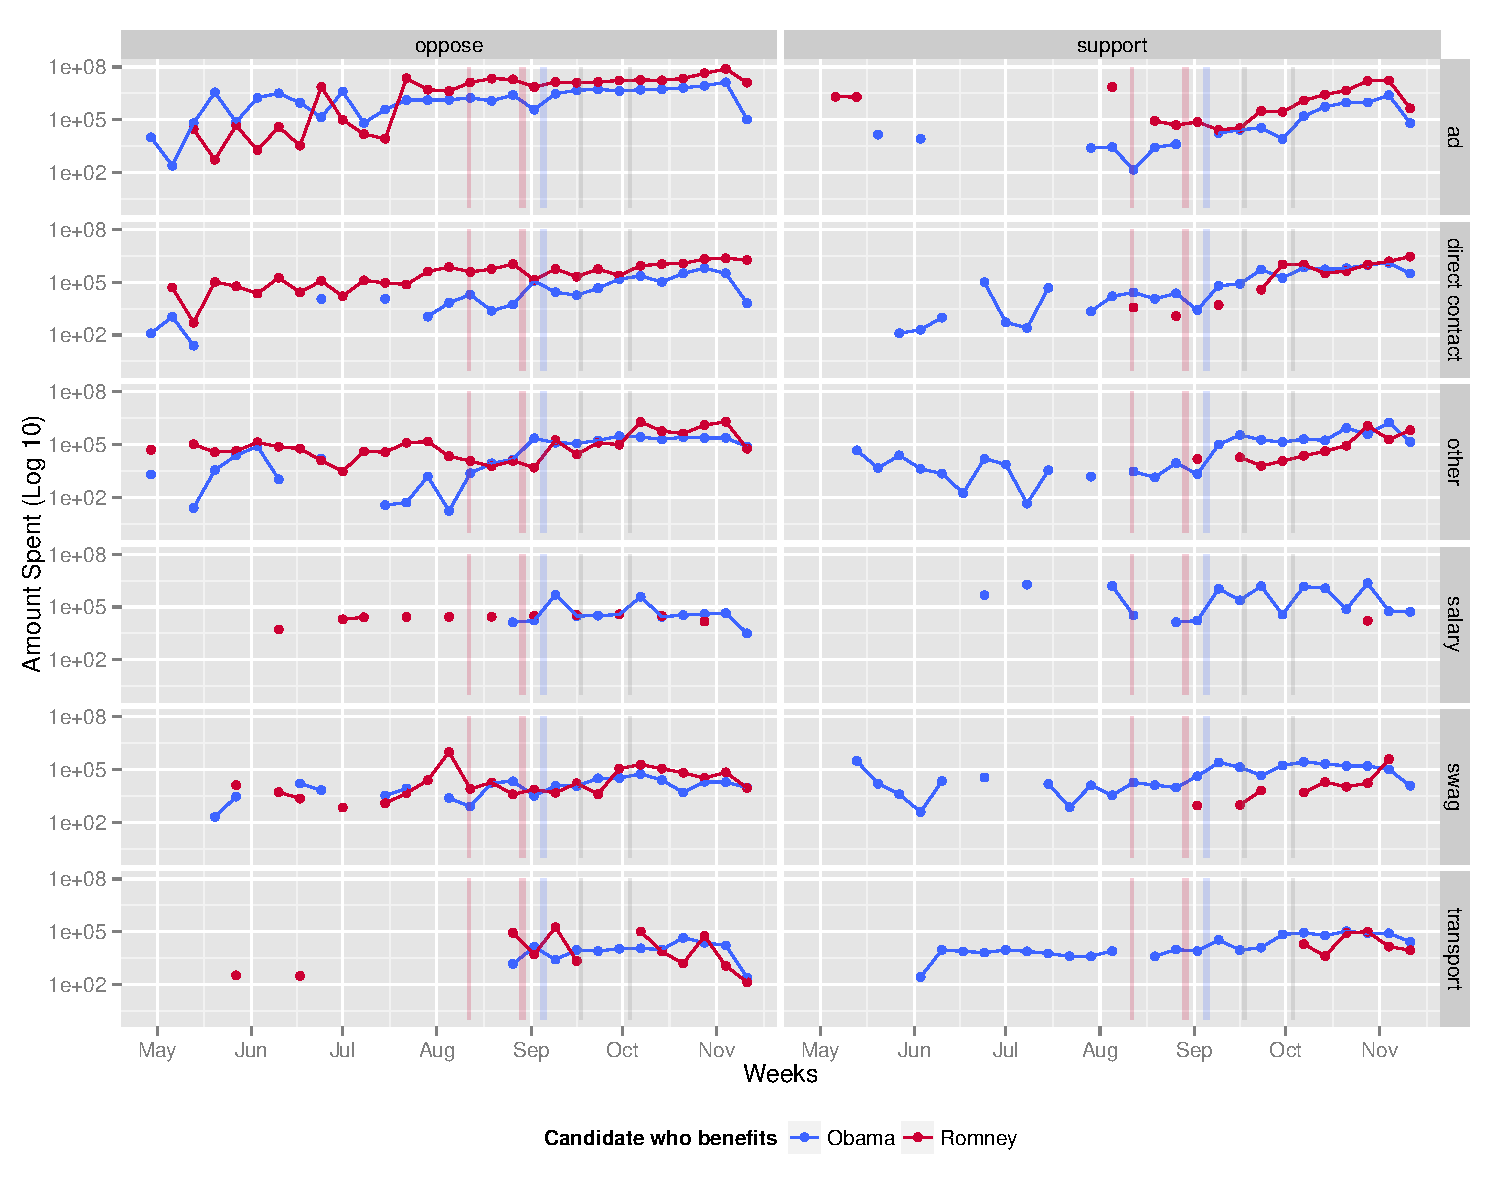
\includegraphics[width=\textwidth]{figure/temporal_plot} 

}

\caption[Spending by Super PACs in support or opposition of candidates]{Spending by Super PACs in support or opposition of candidates\label{fig:temporal_plot}}
\end{figure}

\end{knitrout}



\subsection{Spending Categories}
These plots shows the comparison of amount spent for each candidate by categories of independent expenditure, since April 25, 2012. The categories are mined from the self-reported text description of the expense. The left plot shows the spending to benefit Mr. Obama against the spending to benefit Mr. Romney by category, with values to the right of the reflection line showing PACs supporting Mr. Romney are outspending PACs supporting Mr. Obama on these categories, and vice verse for those to the left. The right plot shows bar chart comparisons of the spending in main categories, on a log scale.
%, and bar charts showing overall spending by amount and by frequency. 
Organizations supporting Romney are greatly outspent those supporting Obama, and particularly in direct contact and advertisements. On the other hand, organizations supporting Obama only outspent those supporting Romney in salary. 
%Organizations supporting Romney are spending a few large chunks of change, but those supporting Obama are spending more frequently and smaller amounts.

\begin{knitrout}
\definecolor{shadecolor}{rgb}{0.969, 0.969, 0.969}\color{fgcolor}\begin{figure}[H]


{\centering 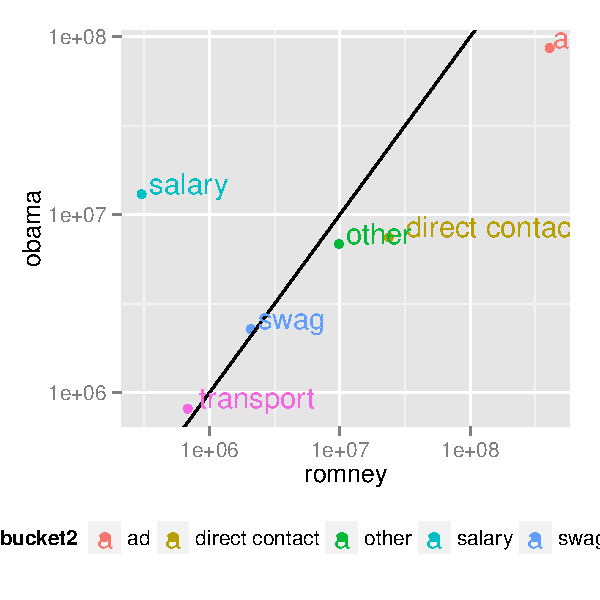
\includegraphics[width=.4\textwidth]{figure/type_plot1} 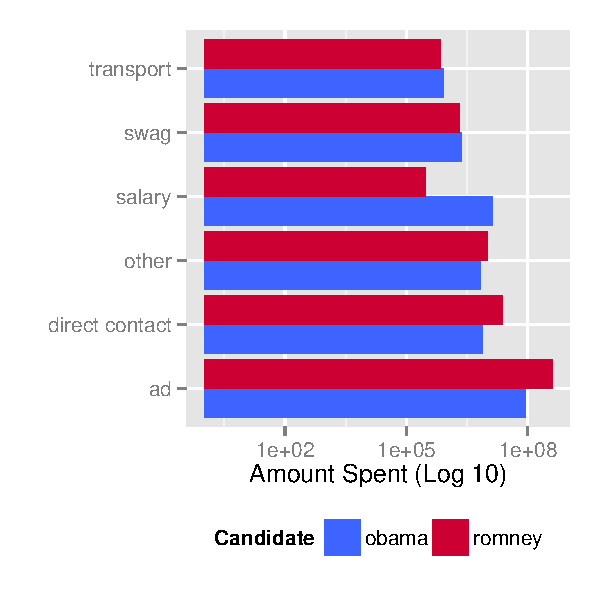
\includegraphics[width=.4\textwidth]{figure/type_plot2} 

}

\caption[Types of spending by category for Romney and Obama Super PACs]{Types of spending by category for Romney and Obama Super PACs\label{fig:type_plot}}
\end{figure}

\end{knitrout}


\subsection{Spending by Independent Organizations}
This chart displays the total spending by the top independent organizations split by candidate. The cumulative amounts spent is displayed vertically, by the benefiting candidate. The organizations supporting Romney have spent significantly more than those for Obama. In fact, two Romney Super PACs (Restore our Future, Inc and Americans for Prosperity) have spent more than all the organizations supporting Obama combined.

\begin{knitrout}
\definecolor{shadecolor}{rgb}{0.969, 0.969, 0.969}\color{fgcolor}\begin{figure}[H]


{\centering 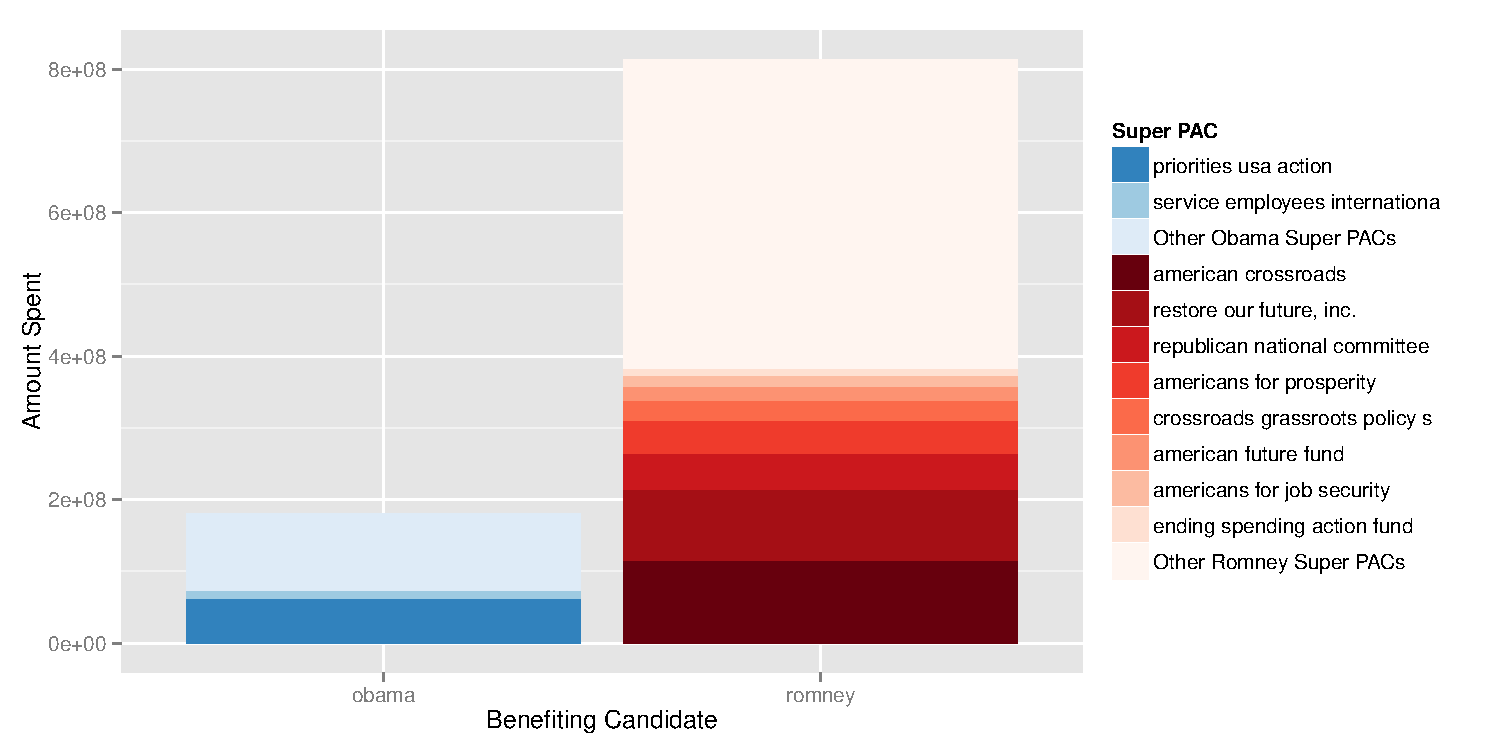
\includegraphics[width=\textwidth]{figure/PAC_plot} 

}

\caption[Spending by Super PAC, stacked by candidate]{Spending by Super PAC, stacked by candidate\label{fig:PAC_plot}}
\end{figure}

\end{knitrout}




\subsection{Swing State Trends}

This plot displays the change in polling support for both Romney and Obama over time, in 12 swing states. The data includes all polls in the National Polls database from April 25th to now. Vertical lines indicate difference between the two candidates, and color shows who is ahead. There are five markers which signify major events in the campaign: the selection of Paul Ryan as Mitt Romney's vice presidential nominee, the Republican National Convention, the Democratic National Convention, the 47\% video and the first presidential debate. 
The plots suggest that the reaction to these major campaign events was not consistent state to state. Some states, such as Wisconsin, have produced drastic changes in polling support over time (``bounces"), while others, such as North Carolina, have maintained a consistent margin of support for the two candidates.

\begin{knitrout}
\definecolor{shadecolor}{rgb}{0.969, 0.969, 0.969}\color{fgcolor}\begin{figure}[H]


{\centering 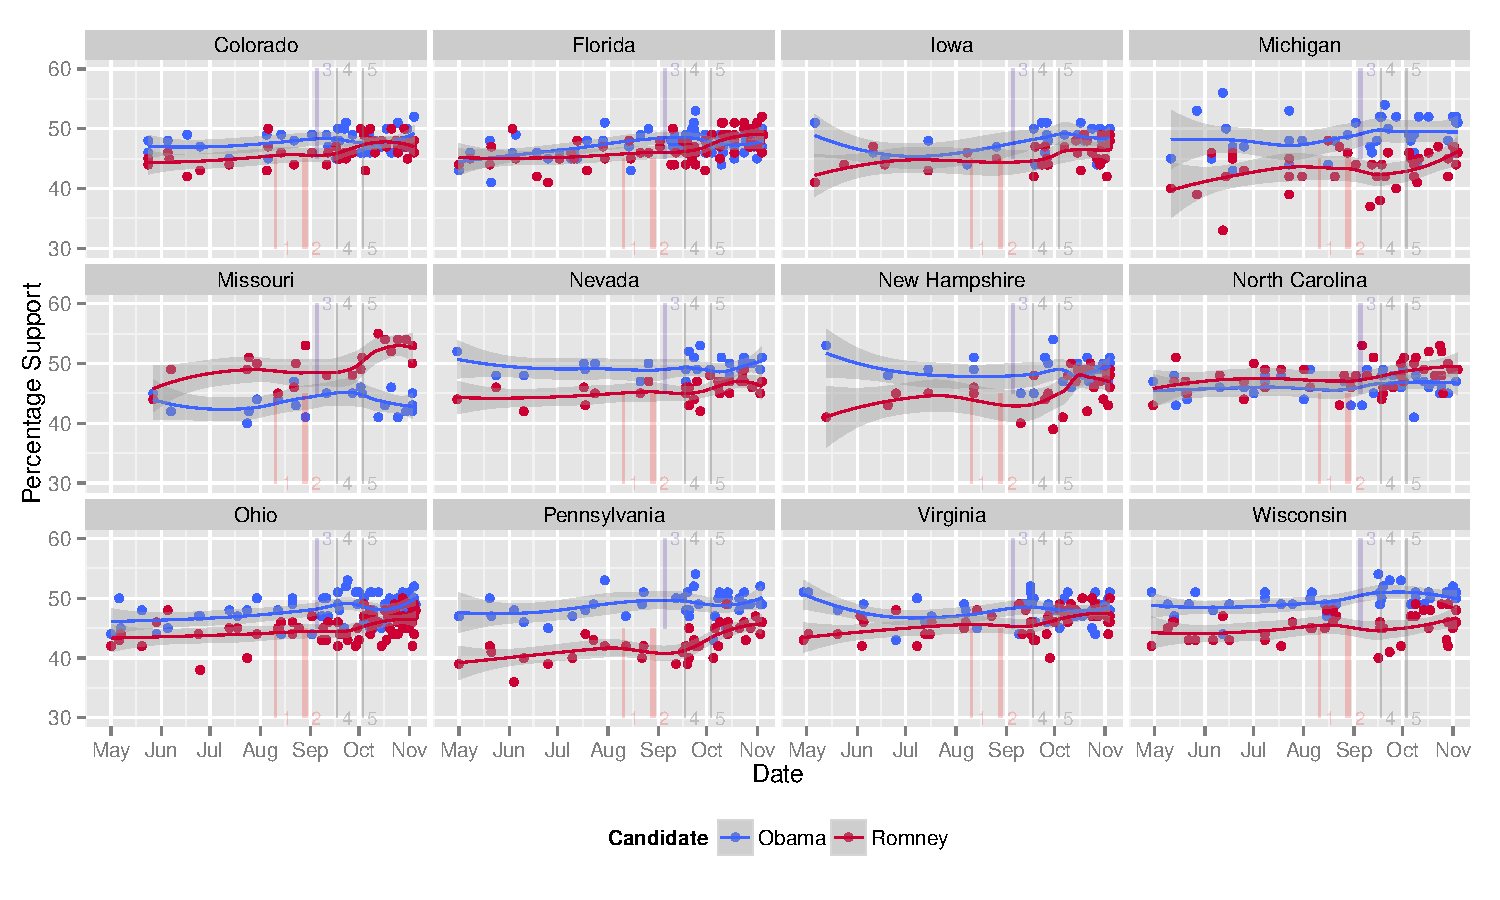
\includegraphics[width=\textwidth]{figure/type_swing_1} 

}

\caption[Polling Averages for Obama and Romney by swing state]{Polling Averages for Obama and Romney by swing state\label{fig:type_swing_1}}
\end{figure}

\end{knitrout}



\subsection{Spending By Week}

Looking at weekly spending by PACs benefiting Romney, we can see a sharp increase in spending that occurred during the week of July 18th. Similarly, there was a sharp increase in spending by Obama-supporting PACs during the week of September 9th. We look at the national and swing-state polls to determine if there is any noticeable effect due to these changes in spending.

\begin{knitrout}
\definecolor{shadecolor}{rgb}{0.969, 0.969, 0.969}\color{fgcolor}\begin{figure}[H]


{\centering 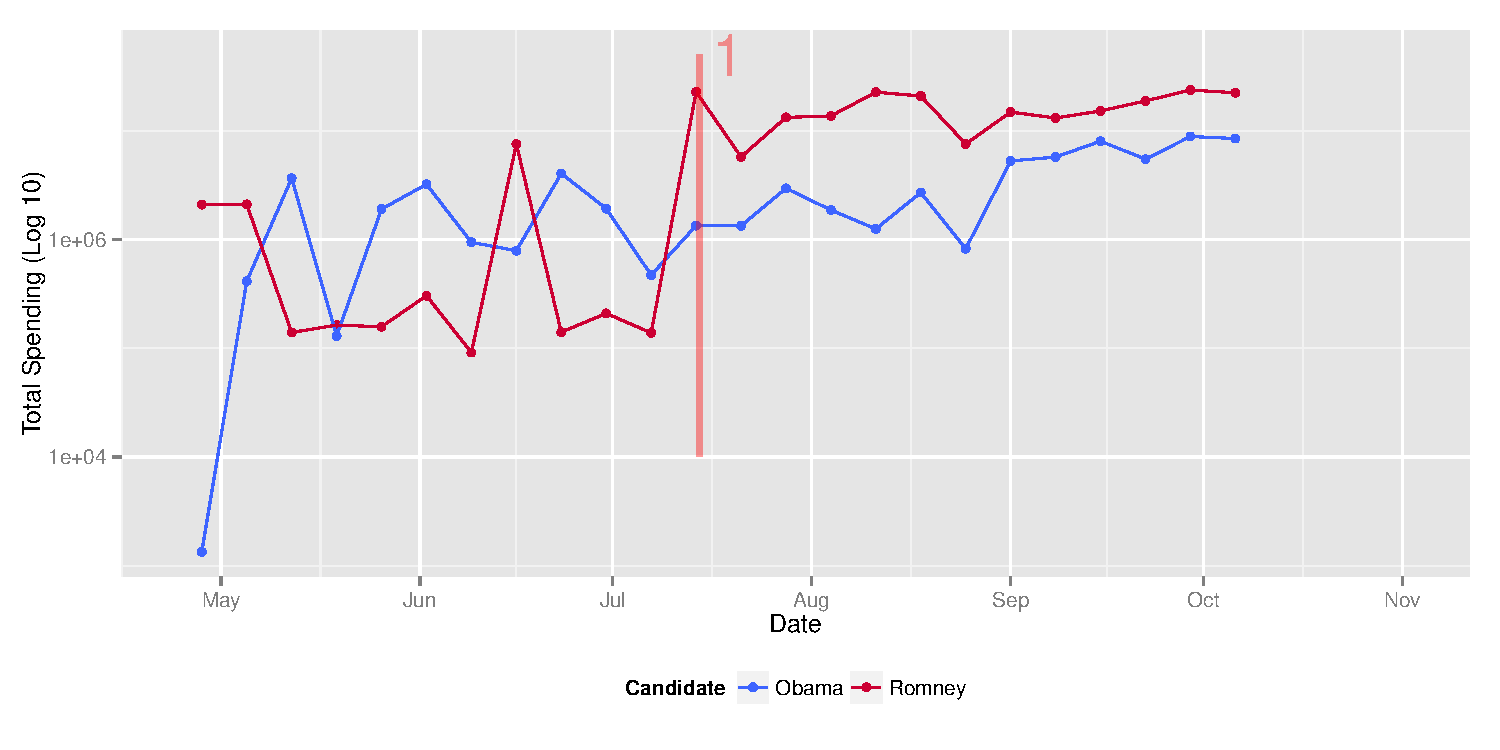
\includegraphics[width=\textwidth]{figure/trend_plot} 

}

\caption[Weekly Spending by Super PACs supporting Obama and Romney]{Weekly Spending by Super PACs supporting Obama and Romney\label{fig:trend_plot}}
\end{figure}

\end{knitrout}


\subsection{Effect of Spending on Polls}

This plot shows the polling margin (Obama - Romney) over time, colored by swing states versus the national polls. It can be seen that Mr. Obama consistently maintained an advantage in swing states relative to his national numbers. A marker is placed on July 18th, corresponding to the sharp increase in spending by Romney-supporting PACs. It does not seem that this spending increase had a measurable effect on the overall trend in the polls at this time.

\begin{knitrout}
\definecolor{shadecolor}{rgb}{0.969, 0.969, 0.969}\color{fgcolor}\begin{kframe}


{\ttfamily\noindent\itshape\textcolor{messagecolor}{\#\# \\\#\# Attaching package: 'zoo'}}

{\ttfamily\noindent\itshape\textcolor{messagecolor}{\#\# The following object(s) are masked from 'package:base':\\\#\# \\\#\#     as.Date, as.Date.numeric}}

{\ttfamily\noindent\itshape\textcolor{messagecolor}{\#\# Loading required package: parallel}}

{\ttfamily\noindent\itshape\textcolor{messagecolor}{\#\# Loading required package: tseries}}

{\ttfamily\noindent\itshape\textcolor{messagecolor}{\#\# Loading required package: fracdiff}}

{\ttfamily\noindent\itshape\textcolor{messagecolor}{\#\# Loading required package: Rcpp}}

{\ttfamily\noindent\itshape\textcolor{messagecolor}{\#\# Loading required package: RcppArmadillo}}

{\ttfamily\noindent\itshape\textcolor{messagecolor}{\#\# Loading required package: colorspace}}

{\ttfamily\noindent\itshape\textcolor{messagecolor}{\#\# Loading required package: nnet}}

{\ttfamily\noindent\itshape\textcolor{messagecolor}{\#\# Loading required package: caret}}

{\ttfamily\noindent\itshape\textcolor{messagecolor}{\#\# Loading required package: lattice}}

{\ttfamily\noindent\itshape\textcolor{messagecolor}{\#\# Loading required package: reshape}}

{\ttfamily\noindent\itshape\textcolor{messagecolor}{\#\# \\\#\# Attaching package: 'reshape'}}

{\ttfamily\noindent\itshape\textcolor{messagecolor}{\#\# The following object(s) are masked from 'package:reshape2':\\\#\# \\\#\#     colsplit, melt, recast}}

{\ttfamily\noindent\itshape\textcolor{messagecolor}{\#\# The following object(s) are masked from 'package:plyr':\\\#\# \\\#\#     rename, round\_any}}

{\ttfamily\noindent\itshape\textcolor{messagecolor}{\#\# The following object(s) are masked from 'package:lubridate':\\\#\# \\\#\#     stamp}}

{\ttfamily\noindent\itshape\textcolor{messagecolor}{\#\# Loading required package: cluster}}

{\ttfamily\noindent\itshape\textcolor{messagecolor}{\#\# Loading required package: foreach}}

{\ttfamily\noindent\itshape\textcolor{messagecolor}{\#\# This is forecast 4.00}}

{\ttfamily\noindent\bfseries\textcolor{errorcolor}{\#\# Error: object 'polls.avg.Nat' not found}}

{\ttfamily\noindent\bfseries\textcolor{errorcolor}{\#\# Error: object 'polls.avg.Swing' not found}}

{\ttfamily\noindent\bfseries\textcolor{errorcolor}{\#\# Error: object 'polls.avg.Nat.Smooth' not found}}

{\ttfamily\noindent\bfseries\textcolor{errorcolor}{\#\# Error: object 'polls.avg.smooth' not found}}

{\ttfamily\noindent\bfseries\textcolor{errorcolor}{\#\# Error: object 'polls.avg.smooth' not found}}

{\ttfamily\noindent\bfseries\textcolor{errorcolor}{\#\# Error: object 'polls.smooth' not found}}

{\ttfamily\noindent\bfseries\textcolor{errorcolor}{\#\# Error: object 'polls.smooth' not found}}

{\ttfamily\noindent\bfseries\textcolor{errorcolor}{\#\# Error: object 'polls.smooth' not found}}

{\ttfamily\noindent\bfseries\textcolor{errorcolor}{\#\# Error: object 'polls.smooth' not found}}

{\ttfamily\noindent\bfseries\textcolor{errorcolor}{\#\# Error: object 'polls.smooth' not found}}

{\ttfamily\noindent\bfseries\textcolor{errorcolor}{\#\# Error: object 'polls.smooth' not found}}\end{kframe}
\end{knitrout}


This plot compares the difference in spending by week by the PACs to the difference in polling between Mitt Romney and Obama with a one week lag. The points are colored by week and certain weeks are labeled to indicated important events. The goal is to see if there is a relationship between PAC spending and poll results. 
In both Obama-supporting and Romney-supporting PACs we can see a weak positive relationship between spending and polling.

\begin{knitrout}
\definecolor{shadecolor}{rgb}{0.969, 0.969, 0.969}\color{fgcolor}\begin{figure}[H]
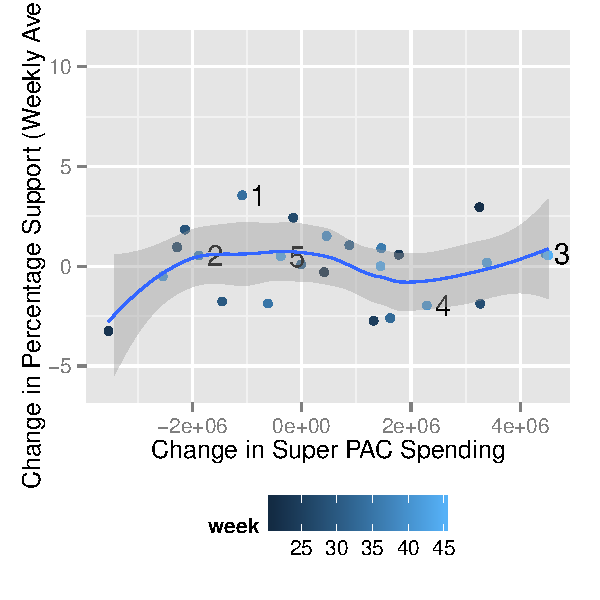
\includegraphics[width=.45\textwidth]{figure/support_spend1} 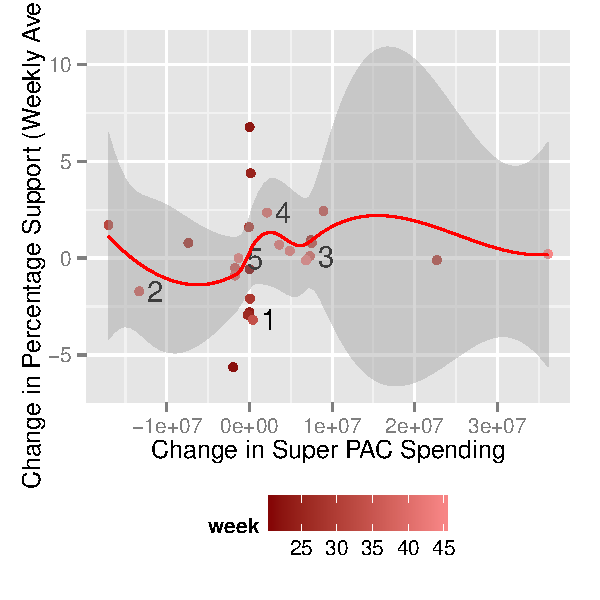
\includegraphics[width=.45\textwidth]{figure/support_spend2} \caption[Change in polling over change in spending by candidate]{Change in polling over change in spending by candidate\label{fig:support_spend}}
\end{figure}

\end{knitrout}


\section{Conclusions/Future Work}
Ultimately, our findings suggest that while election spending itself was a very significant part of the 2012 elections, it is not clear whether the existence of Super PACs had a measurable impact on the outcome. Instead, the events that garnered large amounts of media coverage, such as the 47\% video and the first presidential debate, seemed to have the most noticeable effect on the polling.Furthermore, our analysis did not take into account the spending done by the candidates themselves. It may be that such spending muted the effect of Super PAC spending.

Our analysis also makes clear that Mr. Obama's polling held up more strongly in the swing states than in the national polling throughout the campaign. This advantage was evident in the election results, as well. According to the current AP vote tally as of November 16th, Mr. Obama won the overall popular vote by 2.8\%. But he won Colorado, the state that put him over the 270 electoral votes needed for victory, by 4.7\%. This suggests that Mr. Obama could have lost the popular vote by nearly 2\% and still have been elected president of the United States.

An extension of this project should take into account spending done by the candidates themselves, in addition to independent expenditures. This would allow for a more informed look at the relative spending difference, and how it may or may no correlate with changes in the polling averages. Another area of exploration would be the purpose field of the independent expenditures data set. Our analysis attempted to categorize spending entries into broad categories, but many of the entries in the database have more specific information. For instance, an ad buy may list the name of the ad, as well as the state the ad is running in. It may also be possible to incorporate another data source in order to link the expenditure entries with ad buys in particular states.


\end{document}
